\section{Research Question \& Artefact}

% NEED TO REWRITE THIS SECTION

Through my literature review, there is evidence to show that PCIG should be compared to human designs more frequently to test its authenticity. With this I propose the following research question; \textit{Can an Unknowing Participant distinguish between Multi-Agent Designed and Human Designed Interiors?}
\\
Given this, I also propose the following hypotheses to investigate in order to help me answer the research question.

\subsection{Hypotheses}
\begin{enumerate}
    \item When unaware, the Artefact (\italic{M-A System}) is picked more often than Human designed interiors by participants
    \item When notified, the participant is not able to distinguish between Human and Artefact (\italic{M-A System}) interiors
\end{enumerate}

% NEED TO REWRITE THIS SECTION
\subsection{Artefact}
%The artefact is a Multi-Agent (M-A) system that is used to create a room's furniture arrangement where each piece furniture is seen as an individual agent. The individual agents have their own semantic descriptions using Unity's \cite{unity} ScriptableObject class. Within these ScriptableObject's, they have information such as the type of furniture they are, the occupation of each of their sides and what other furniture types they can have as potential parents. The agents are represented in scene using pre-fabricated assets from a free-to-use Unity asset pack by Brick Project Studio \cite{brick-project}.

%\hl{A User must select what furniture they would like to be used within a}

%The system is given an empty room and has access to pre-made furniture assets, at run time agents are spawned and arrange themselves accordingly (the behavior of a singular agent is demonstrated in Fig. ~\ref{activity-diagram}). The artefact will be influenced by the work from \textit{T. Germer, et al.} \cite{real-time-walkthroughs}.

The artefact proposed to help answer my research question is a Multi-Agent (M-A) system that is used to create a room's furniture arrangement where each piece of furniture is seen as an individual agent. These individual agent's use the Unity's \cite{unity} ScriptableObject class to contain all necessary information about themselves. This information includes data such as the type of furniture they are, the occupation of each of their sides and what other furniture types they can have as a potential parent - see Fig~\ref{agent-so} for an example of an Agents ScriptableObject. The agents are represented in a scene using pre-fabricated assets from a free-to-use Unity asset pack by Brick Project Studio \cite{brick-project}.

To generate a room's layout, the agents must have access to an empty room. In order for the furniture to be arranged, a user must place the furniture that they want to be placed in the Unity scene. Once the scene is running, the agents handle and place themselves accordingly within the room.
All agents begin in a \italic{SEARCH} state, within this state the agent aims to find a potential parent that is defined within its ScriptableObject. Once a parent is found, the agent begins its \italic{ARRANGE} state where it places and orients itself appropriately. Once placed, the agents state changes to \italic{REST}. The behaviour of a singular agent used in the Artefact is also demonstrated in Fig.~\ref{activity-diagram}.
The behaviour behind the agents in the artefact is influenced by the work from \textit{T. Germer, et al.} \cite{real-time-walkthroughs}.

\begin{figure}[!ht]
    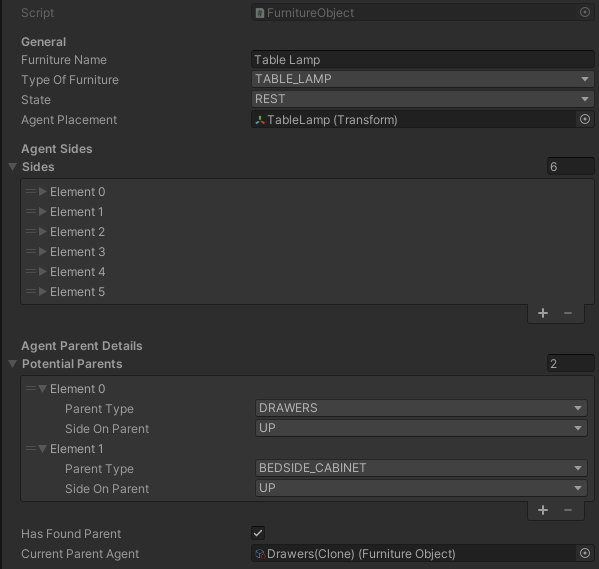
\includegraphics[width=\columnwidth]{./Images/agent-SO.png}
    \centering
    \caption{Screenshot of an agent's ScriptableObject}
    \label{agent-so}
\end{figure}

% NEED TO REWRITE THIS SECTION
\subsection{Artefact Development \& Quality Assurance} 
For the implementation of the Artefact, the Unity Game Engine \cite{unity} was used as I have used this engine throughout my time at University and have thorough experience with using this engine in creating both small and large projects. Furthermore, the knowledge I have in the C\# language and Unity's base classes helped further in deciding what engine to use for the Artefact.
Throughout the Artefact's development life-cycle, I also closely followed an Agile methodology and it's principles to help me slowly but iteratively develop a finished product. Using Agile to help with the artefact's development was a clear choice for me as it is commonly used in Software Engineering and Game Development environments alike \cite{game-dev-agile}, but I have also followed this methodology closely throughout my time at University, using it when working on other small or large projects. I worked in bi-weekly sprints and set myself achievable tasks in-order for my Artefact to progress further along in its development.
\\
Throughout the Artefact's development, along with Agile, it was continuously tested using Unity's Test Framework \cite{unit-unit-testing} and C\#'s \italic{NUnit Framework}\cite{nunit-framework} and a pilot test was conducted to ensure the research methodology of this dissertation. (More details of Unit testing and the Pilot test can be found in \hyperref[append:f]{Appendix F}).